\documentclass[a4paper,12pt]{article}
%\documentclass[a4paper,12pt]{scrartcl}

\usepackage{xltxtra}

\input{../preamble.tex}

\usepackage[spanish]{babel}

% \setromanfont[Mapping=tex-text]{Linux Libertine O}
% \setsansfont[Mapping=tex-text]{DejaVu Sans}
% \setmonofont[Mapping=tex-text]{DejaVu Sans Mono}

\title{Tarea \#01}
\author{Isaac Ayala Lozano}
\date{2020-02-19}

\usepackage{fancyhdr}

\pagestyle{fancy}
\fancyhf{}
\rhead{Visión por Computadora  \hspace{2 em}}
\lhead{Isaac Ayala Lozano}
\fancyfoot[R]{\thepage}


\begin{document}
\maketitle

\begin{enumerate}
 \item Se presentan las observaciones para cada imagen.

 \begin{table}[htb!]
  \begin{center}
\begin{tabular}{lcccc}
 & Figura 1 & Figura 2 & Figura 3 & Figura 4\\
Axioma 1 & $\checkmark$ & $\checkmark$ & $\checkmark$ & $\checkmark$\\
Axioma 2 & $\checkmark$ & $\checkmark$ & $\checkmark$ & $\checkmark$\\
Axioma 3 & $\checkmark$ & $\checkmark$ & $\checkmark$ & $\checkmark$\\
Axioma 4 & $\checkmark$ & $\checkmark$ & $\checkmark$ & $\checkmark$
  \end{tabular}
  \end{center}
 \end{table}


    \begin{itemize}
     \item La figura 1 cumple con los cuatro axiomas de geometría proyectiva.
     Es posible identificar a dos puntos de fuga en la imagen.
     A pesar de tener en mayor proporción las curvas que debido a las formas orgánicas del paisaje.
     \item La figura 2 posse un único punto de fuga ubicado en el centro de la imagen.
     La imagen cumple con los cuatro axiomas de la geometría proyectiva.
     \item La figura 3 presenta al menos dos puntos de fuga. Hay un punto de fuga en cada lado de la figura.
     Cumple tambień con los cuatro axiomas de la geometría proyectiva.
     \item La figura 4 corresponde a la obra \emph{Satire on False Perspective} por William Hogarth.
     La figura cumple con los axiomas de la geometría proyectiva.
     Las características de la imagen la vuelven un \emph{objeto imposible}.
     Existen múltiples detalles en la escena, que vuelven imposible la existencia del objecto.
    \end{itemize}
 \item Los dibujos se encuentran en el apéndice.
 \item Sistema de visión de la familia de cefalópodos: Nautilus.
\end{enumerate}


\section{Sistema de visión - Nautilus pompilus}

La especie de Nautilus pompilus posee un sistema de visión centrado en el concepto de \emph{cámara obscura}\footnote{del latín camera obscūra}.
El ojo de esta especie, y del género de Nautilus en general, carece de un lente \cite{sasaki2010Anatomy} para enfocar los rayos de luz.
En vez de esto posee un ojo rudimentario con una pupila (pu en figura \ref{fig: electron microscope}) en forma de un agujero diminuto que permite el paso de luz hacia la retina (figura \ref{fig: pinhole eye}).


\begin{figure}[hbt!]
 \centering
 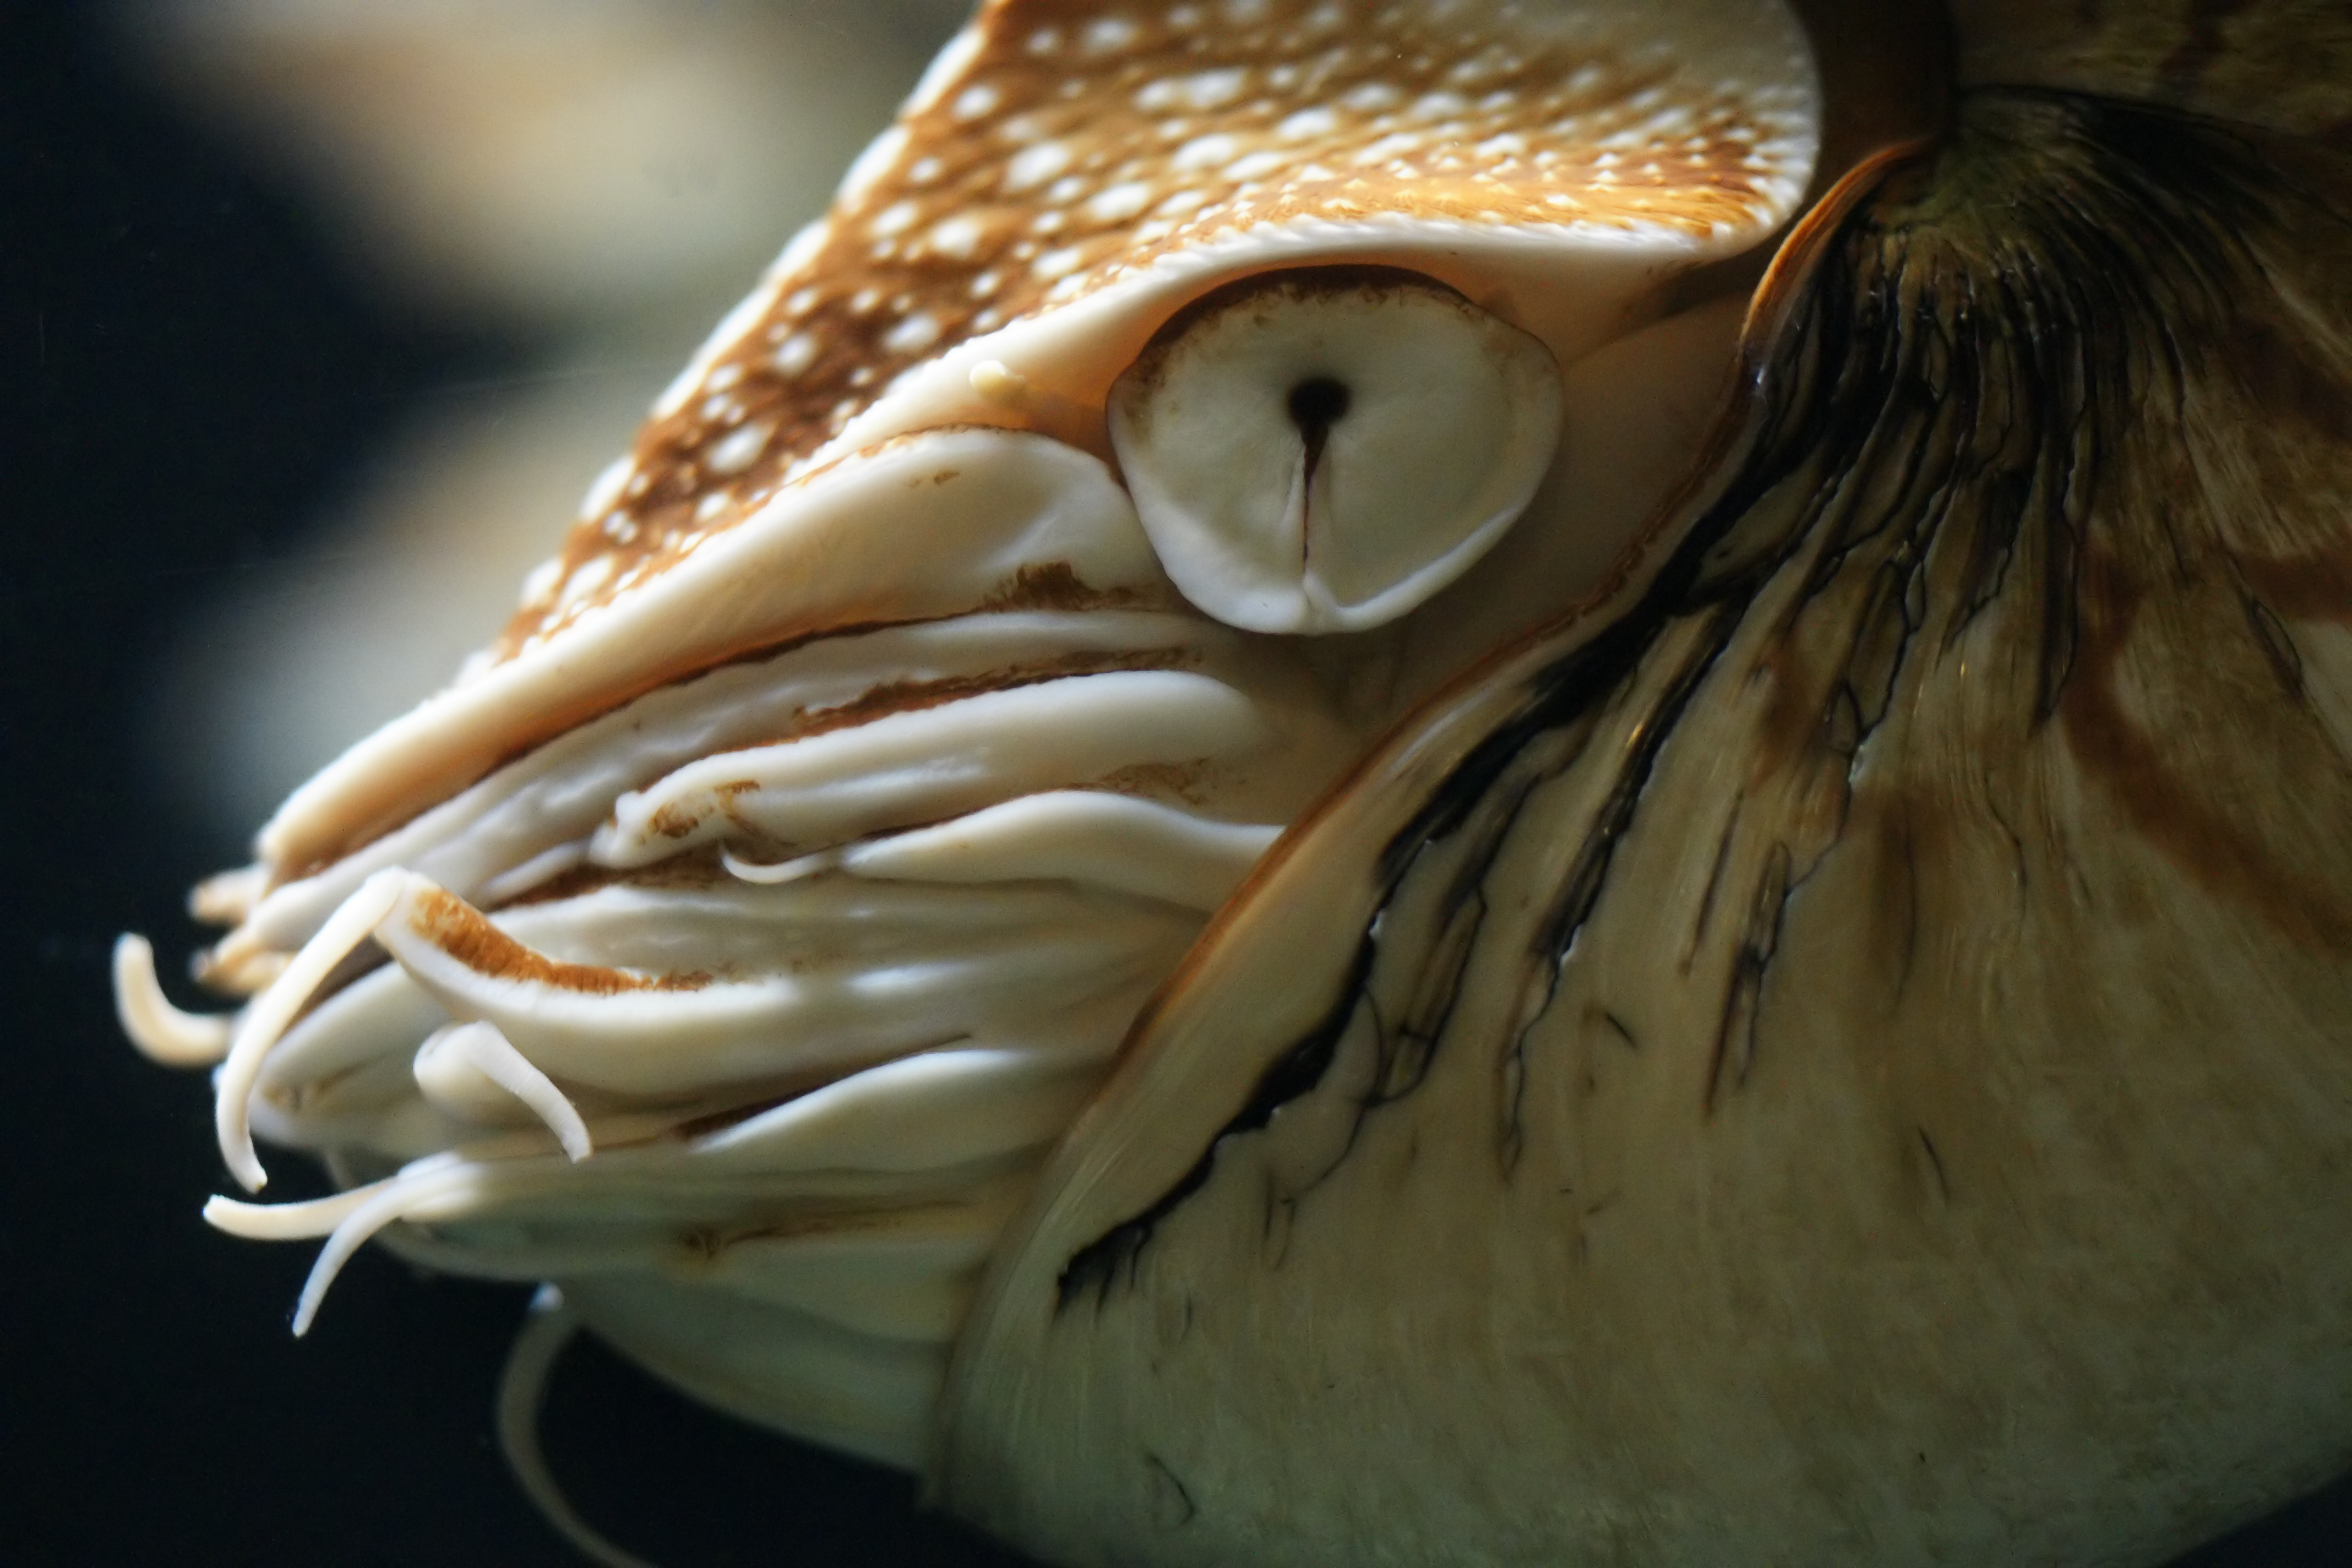
\includegraphics[width=\textwidth]{Nautilus_pompilius_eye}
 \caption{Ojo rudimentario de Nautilus pompilus. Cortesía de \cite{hillewaert2008Nautilus}}
 \label{fig: pinhole eye}
\end{figure}

\begin{figure}[hbt!]
 \centering
 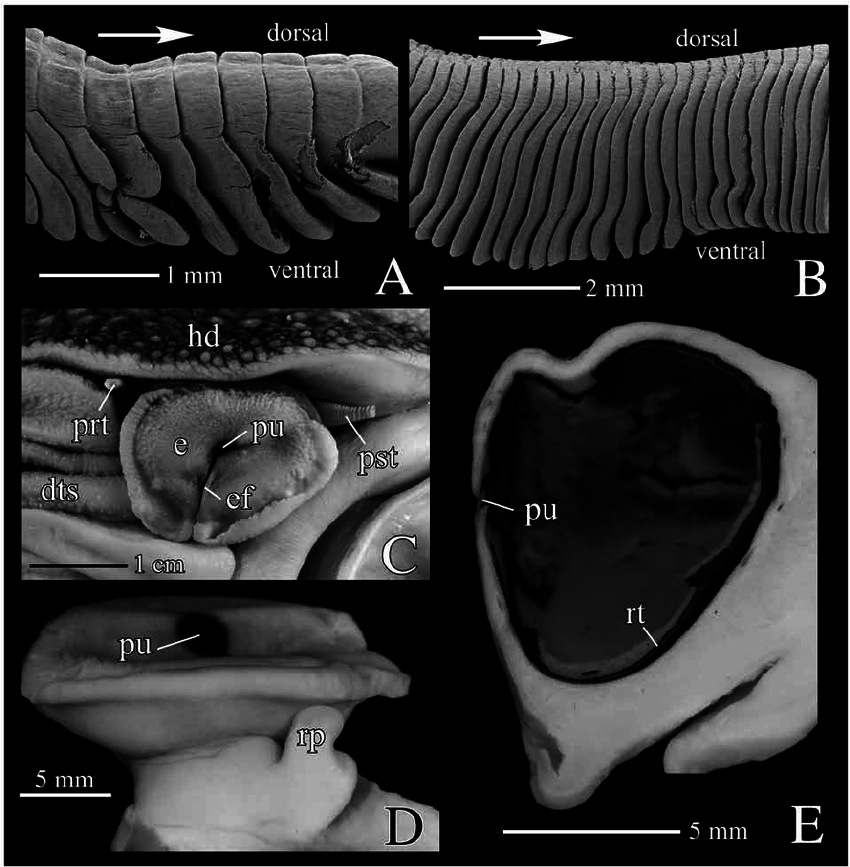
\includegraphics[width=\textwidth]{Nautilus-pompilius-Linnaeus-Sense-organs}
 \caption{Vista detallada del ojo (C). Cortesía de \cite{sasaki2010Anatomy}}
 \label{fig: electron microscope}
\end{figure}


Se presenta en la figura \ref{fig: retina} la forma y tamaño aproximado del ojo del Nautilus pompilus de acuerdo a \cite{muntz1984VisualSystem}.

\begin{figure}[hbt!]
 \centering
 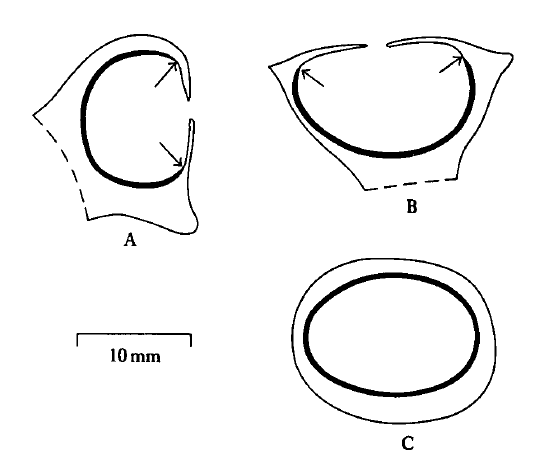
\includegraphics[width=\textwidth]{nautilus_retina}
 \caption{Forma y dimensiones del ojo. (A) Sección vertical, (B) sección horizontal, (C) vista del fondo de ojo. En (A) y (B) las flechas indican los límites de la retina, mostrada en negro. \cite{muntz1984VisualSystem}}
 \label{fig: retina}
\end{figure}



De \cite{muntz1984VisualSystem} es sabido que la calidad de imagen que la especie puede percibir de su entorno es inferior a la de otras especies de la familia de cefalópodos.
El principio del funcionamiento de la cámaro obscura es uno de los principales causantes.
Se especula que el género de Nautilus hace uso de otros sentidos para guiarse, dejando de lado el sentido de la vista.
En el estudio realizado por Muntz se construyeron tres modelos del ojo de la especie para determinar la resolución y calidad de la imagen, los resultados pueden observarse en la figura \ref{fig: resolution}.

\begin{figure}[hbt!]
 \centering
 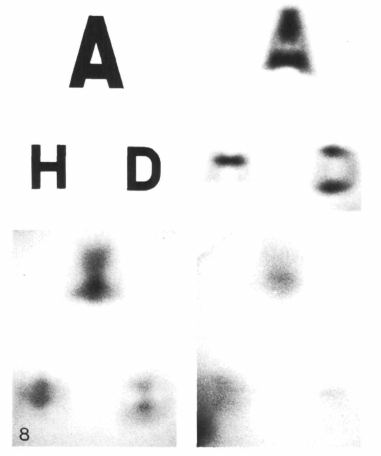
\includegraphics[width=\textwidth]{nautilus_resolution}
 \caption{Fotografías tomadas a través de los modelos de ojo con pupilas horizontales de diferentes tamaños. La imagen en la esquina superior izquierda muestra el diagrama empleado y las demás imágenes los resultados de cada modelo. \cite{muntz1984VisualSystem}}
 \label{fig: resolution}
\end{figure}



% https://en.wikipedia.org/wiki/File:Nautilus_pompilius_(head).jpg

% https://en.wikipedia.org/wiki/File:Nautilus_diagram-en.svg

% https://jeb.biologists.org/content/109/1/253.short

\clearpage

\printbibliography

\end{document}
